%%%%%%%%%%%%%%%%%%%%%%5
\graphicspath{{}{nustorm/}{Diagrams/}}

Neutrinos from STORed Muons ($\nu$STORM) is an experimental proposal for a non-conventional but well-understood neutrino beam from the decay of stored muons. The energy range and the small uncertainties in the flux normalisation make \nus the ideal place to measure neutrino-nucleon cross sections. This can serve as a crucial input for long-baseline physic~\cite{Soler2015}, increasing the sensitivity of future experiments to CP violation and other oscillation parameters. In addition, it provides a clean and intense environment to look for new physics in accelerator neutrino beams. One immediate application is to search for light sterile neutrinos~\cite{Adey:2013pio,Adey:2014rfv}, either via short-baseline oscillations or via short-distance flavour transitions. In this chapter, we will explore this topic emphasizing the two detector setup for \nus and its sub-percent flux uncertainties. \nus was originally proposed as a facility to be based at Fermilab, using 60 GeV protons~\cite{Adey:2013pio}. This design, however, is currently being adapted for siting at CERN instead. At the time of writing, no further developments in terms of ring design and detector considerations has been agreed on. This work is based mostly on the original design of Ref.~\cite{Adey:2013pio}, with a few modifications we clarify below. 

\section{\nus}
%
\begin{figure}[t]
\centering
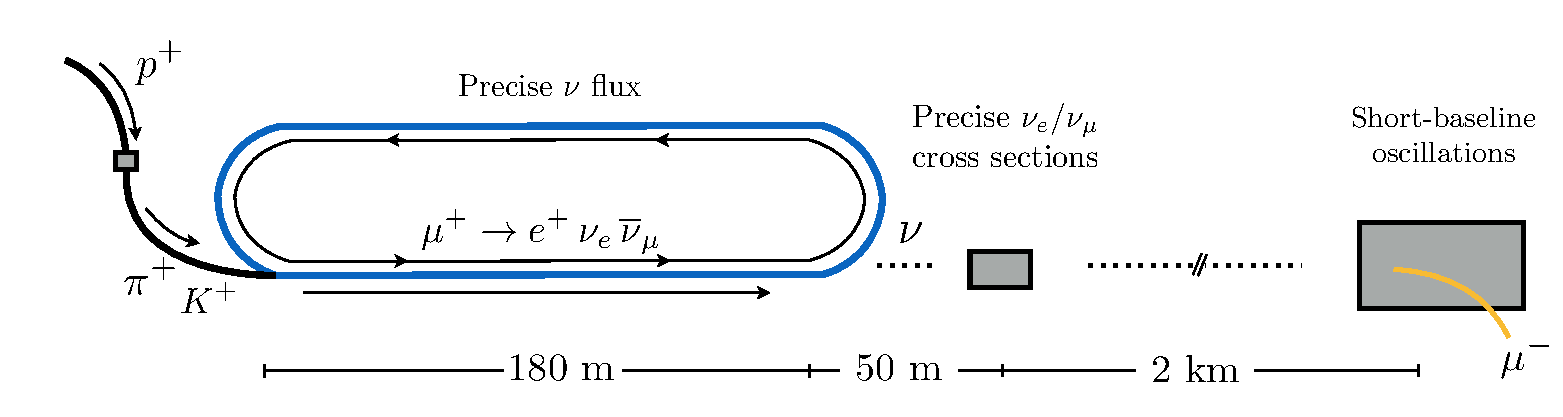
\includegraphics[width=\textwidth]{nustorm.pdf}
\caption[The \nus setup in a diagramatic representation.]{\nus in a diagram. \label{fig:nustorm_diagram}}
\end{figure}
%

The neutrino beam at \nus is derived from the decay of pions and stored muons. \nus is an accelerator neutrino experiment, and so relies on meson production in the usual way: high-energy protons colliding onto a solid target. A magnetic horn then collects $5.0 \pm 0.5$ GeV charged pions of the desired polarity, and inject them in the first straight of a racetrack like storage ring, where $52$\% of the collected charged pions are expected to decay before being stopped at the end of the straight. Muons with an energy of $3.8 \pm 0.38$ GeV are then collected and stored in the ring, where they are expected to circulate for a mean number of 50 turns. The first straight section of the ring, the decay pipeline, is estimated to be $180$ m long~\cite{Neuffer2015}, which will determine the size of the neutrino production region. 
In this setup, one obtains a beam of  $\nu_{\mu}$ ($\overline{\nu}_{\mu}$) from the decays of the injected $\pi^+$ ($\pi^-$) in what we call the \emph{pion flash}. The useful decays of the stored $\mu^+$ ($\mu^-$) then yield a beam of $\overline{\nu}_{\mu}$ ($\nu_{\mu}$) and $\nu_e$ ($\overline{\nu}_{e}$). The injection of pions into the ring is assumed to happen at large enough time intervals to allow for a discrimination between the neutrinos coming from the pion flash and the ones coming from the useful muon decays (a timing cut of the order of $180/c = 600$ ns or greater is needed to account for all pion decays before the muon data collection~\cite{Tunnell2013}). This allows us, for example, to completely separate the oscillations channels involving $\nu_{e}$ and $\overline{\nu}_{\mu}$ from the ones involving $\nu_{\mu}$ as initial states, for the $\pi^+$ polarity. It is clear, however, that a small contamination of muon decays happens during the pion flash. This is a small number of the neutrinos produced, and is taken into account by including $1\%$ of the muon decay flux into the pion flash neutrino flux. Kaons also contribute to the pion flash flux, albeit at larger energies~\reffig{fig:nustorm_flux}. 
%
\begin{figure}[t]
\centering
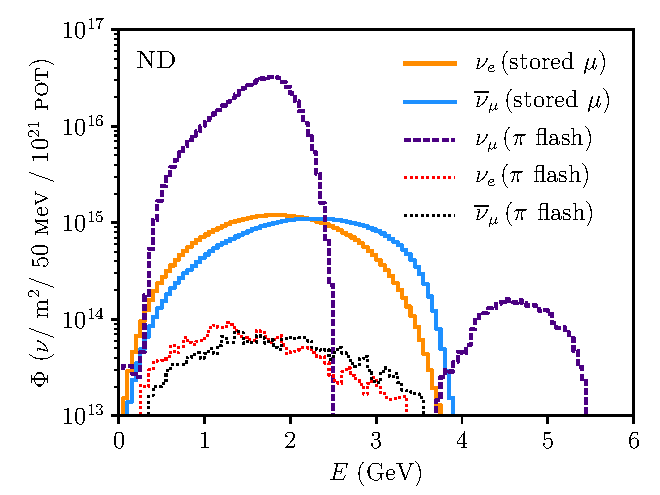
\includegraphics[width=0.49\textwidth]{figs/flux_ND.pdf}
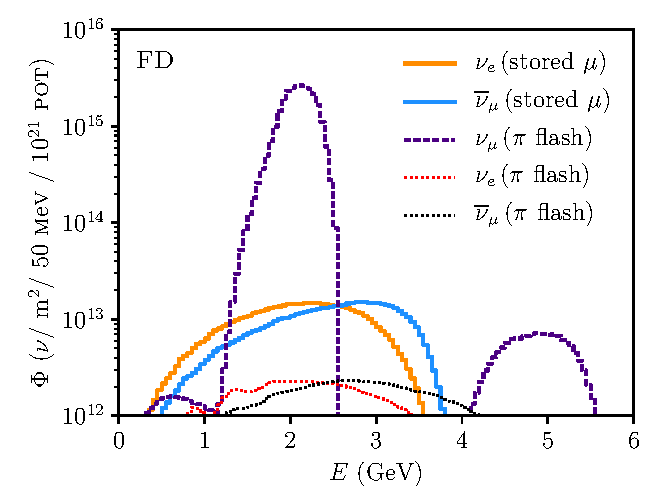
\includegraphics[width=0.49\textwidth]{figs/flux_FD.pdf}
\caption[The \nus neutrino flux for the near and far detector.]{The neutrino flux at the near (left) and far (right) detectors of \nus. Note that the neutrinos from stored muons are separated from the ones generated in the pion flash through timing. \label{fig:nustorm_diagram}}
\end{figure}
%


\subsection{3+N short-baseline oscillations}
%
Standard Model neutrinos produced in charged current interactions are flavour eigenstates $\nu_{\alpha}$ ($\alpha = e,\mu$ or $\tau$). The misalignment between the flavour eigenstates $\ket{\nu_{\alpha}}$ and the mass eigenstates $\ket{\nu_i}$ in the presence of non-degenrate masses is responsible for neutrino oscillations and mixing. The mixing is described by a matrix $U$, which in the case of 3 active neutrinos is given by the $3 \times 3$ Pontecorvo-Maki-Nakagawa-Sakata (PMNS) matrix. In general, for $3+N$ flavour and $3+N$ mass eigenstates, we have
%
\begin{equation} \label{eq:mixing}
\ket{\nu_{\alpha}} = \sum_{i}^{3+N} U_{\alpha i}^* \ket{\nu_{i}}.
\end{equation}   
%
The invisible decay width of the Z boson as measured at LEP \cite{Schael2006} indicates that there are only 3 weakly interacting neutrino states. The $N$ additional flavour eigenstates will be referred to as sterile states, as these are singlets under all SM gauge groups. Similarly, the $N$ additional mass eigenstates are also typically called sterile, since that is their dominant flavour composition.

In general, in a quantum mechanical treatment of neutrino oscillations, the oscillation probability for a neutrino preoduced as a flavour $\alpha$ to be detected as a state $\beta$ can be written as a function of the baseline $L$ and the neutrino energy $E$ as
%
% \begin{equation} \label{eq:general_prob}
% P_{{\alpha {\beta}}}(L, E) = \sum_{j}^{3+N} \sum_k^{3+N} U_{\alpha j}^* U_{\beta j} U_{\alpha k} U_{\beta k}^* \, I_{j k} (L, E),
% \end{equation}    
%
\begin{align} \label{eq:general_prob}
P_{\nu_{\alpha} \to \nu_{\beta}}= \delta_{\alpha \beta} -& 2 \sum_{k>j}^{3+N} \Re(U_{\alpha k}^* U_{\beta k} U_{\alpha j} U_{\beta j}^*)\, \left(1 - \Re\left[I_{k j}(L, E)\right]\right) \nonumber\\ -& 2\sum_{k>j}^{3+N} \Im(U_{\alpha k}^* U_{\beta k} U_{\alpha j} U_{\beta j}^*) \Im\left[I_{k j}(L, E) \right],
\end{align}
where the factor $I_{k j}(L, E)$ satisfies $I_{k k} = 1$ and $I^*_{k j} = I_{j k}$ \cite{Akhmedov2009a} and will contain any information about the coherence of production, propagation and detection of neutrino mass states. More commonly, under the plane-wave approximation and assuming ultra-relativistic neutrinos with $L = t$, this factor is related to the time evolution of the mass eigenstates and reads
%
\begin{equation} \label{eq:Iplanewave}
I_{k j}(L, E) = \exp\left(-i \frac{\Delta m^2_{k j} L}{2 E}\right).
\end{equation}
%
The plane-wave approximation, however, fails to properly accommodate effects due to the finite size of the production or detection region, which might play an important role in oscillations due to steriles with masses above a few eV. In section \ref{sec:prodcoh} we motivate and lay out the necessary formalism developed in \cite{Akhmedov2009,Akhmedov2012} for dealing with these issues.

Equation \ref{eq:mixing} implies that with the addition of $N$ sterile neutrinos the mixing matrix is enlarged to an $N \times N$ matrix. At the short-baselines we are interested in, however, we can safely ignore any terms in the oscillation probability which contain the active mass-squared differences ($\Delta m^2_{31} \approx 7 \times 10^{-5}$ eV$^2 \ll\Delta m^2_{21} \approx 10^{-3}$ eV$^2 \ll \Delta m^2_{\text{SBL}}$). All oscillations (as a special case of flavour transitions) discussed in this paper will be due to active-sterile mass-squared differences $\Delta m^2_{\text{SBL}}$, which are taken to be in the range $10^{-1}$ -- $10^{3}$ eV$^2$. In particular, we will only consider the case where all sterile neutrinos are heavier than the active ones.   

In a 3+1 scenario under the short-baseline approximation, equation \ref{eq:general_prob} gives the following oscillation probability
%
\begin{equation} \label{eq:app3+1}
P^{3+1}_{\nu_{\alpha} \to \nu_{\beta}} = 2 |U_{\alpha 4}|^2 |U_{\beta 4}|^2 \big(1 -\Re(I_{41}) \big)
\end{equation}
%
for appearance, and
%
\begin{equation} \label{eq:dis3+1}
P^{3+1}_{\nu_{\alpha} \to \nu_{\alpha}} = 1 - 2|U_{\alpha 4}|^2(1 - |U_{\alpha 4}|^2) \big(1 -\Re(I_{41}) \big),
\end{equation}
%
for disappearance. In the 3+1 case, it is customary to write the probabilities in terms of the more phenomenological parameters $\sin^2 {2 \theta_{\alpha \beta}} = 4 |U_{\alpha 4}|^2 |U_{\beta 4}|^2 $ and $\sin^2 {2 \theta_{\alpha \alpha}} = 4 |U_{\alpha 4}|^2(1 - |U_{\alpha 4}|^2) $, and we use these througout the paper.

In the presence of two sterile neutrinos at the eV scale, the oscillation is effectively a 3 neutrino case. This means that the probability formula picks up a complex phase, which will be parametrized by $\eta = \arg{(U_{\alpha 5}^* U_{\beta 5} U_{\alpha 4} U_{\beta 4}^*)}$. The short baseline approximation to the probability reads
%
\begin{align}
P^{3+2}_{\nu_{\alpha} \to \nu_{ \beta}}  =\, &2 \left|U_{\alpha 4}\right|^2 \left|U_{\beta 4}\right|^2 \left(1 - \Re(I_{4 1}) \right) + 2 \left|U_{\alpha 5}\right|^2 \left|U_{\beta 5}\right|^2 (1 - \Re(I_{5 1})) \nonumber \\
+ &2 \left| U_{\alpha 4} U_{\beta 4} U_{\alpha 5} U_{\beta 5}\right|  \Re\left[ e^{i \eta} \left( 1 - I_{41}^* - I_{51} + I_{54} \right) \right],
\end{align}
%
for apperance, and
%
\begin{align}
P^{3+2}_{\nu_{\alpha} \to \nu_{ \alpha}}  =\,1 - &2(1 - |U_{\alpha 4}|^2 - |U_{\alpha 5}|^2) \times \left[ |U_{\alpha 4}|^2 \big(1 - \Re(I_{41}))  + |U_{\alpha 5}|^2 \big( 1 - \Re(I_{51}) \big)\right] \nonumber \\ - &2 |U_{\alpha 4}|^2 |U_{\alpha 5}|^2 \left(1 - \Re(I_{54})\right), 
\end{align}
%
for disappearance. Note how the CP complex phase only appears in the appearance formulae since CPT invariance implies CP conservation for the disappearance channel. Full expressions for the oscillation probability in the plane wave approximation can be obtained by using equation \ref{eq:Iplanewave}, and for production decoherence assuming point like parent particles one can use the expressions for $I_{k j}$ as shown in \refapp{sec:appendix_prob}.

%%%%%%%%%%%%%%%%%%%%%%%%%%%%%%%%%%%%%%%%%%%%%%%%%%%%%%%%%%%%%%%%%%%%%%%%%%% 
\subsubsection{Localization at production \label{sec:prodcoh}}

The presence of light sterile neutrinos with masses above the eV scale can realise the interesting scenario where the localization at production might be broken. For a neutrino to be created as a coherent superposition of different mass eigenstates we should not be able to resolve what mass eigenstate was produced, {\it i.e.} $\sigma_{m^2} \gg \Delta m^2$ for all the involved mass-splittings is a condition for production coherence~\cite{Akhmedov2012}. Using the relativistic expression for the neutrino energy, the condition for the uncertainty on the neutrino momentum $\sigma_P$ can be written as
%
\begin{equation}
\sigma_P \gg \frac{\Delta m^2}{2P}.
\end{equation}
%
If we assume that $\sigma_P$ is related to the uncertainty in the spatial coordinate of the neutrino as $\sigma_P \sim \text{\it min} (1/\sigma_{x_S}, 1/\sigma_{x_D})$, we arrive at the well known condition for neutrino oscillations not to be washed-out \cite{Akhmedov2009}
%
\begin{equation}
\sigma_{x_S} \ll L_{\text{osc}}, \quad \sigma_{x_D} \ll L_{\text{osc}},
\end{equation} 
%
where $L_{\text{osc}} = 4 \pi P/\Delta m^2$ and factors of 2 and $\pi$ were ignored. This condition says that the production or detection decoherence effects are equivalent to the averaging of the oscillations due to finite size of sources and detectors.

The production region at \nus, for example, is given by the size of the decay pipeline $\ell_p = 180$ m. This is only an order of magnitude smaller than the far detector baseline ($\approx 2$ km) and, more importantly for higher mass sterile searches, it is larger than the near detector distance from the end of the decay pipeline. For instance, if a sterile neutrino with a mass larger than $10$ eV is present, the near detector would only see flavour transitions constant in energy.

The probabilities derived in the previous section have been derived for a general factor $I_{k j}$, which under the plane-wave approximation is given by equation \ref{eq:Iplanewave}. In the wavepacket treatment for neutrino oscillations, $I_{k j}$ is corrected by production, detection and propagation coherence factors \cite{Akhmedov2009}:
%
\begin{equation}
I_{k j} = \exp\left(-i \frac{\Delta m^2_{k j} L}{2 P}\right) S_{\text{prop}}(L/L^{\rm coh}_{kj}) S_{\text{P/D}}(\sigma_x/L^{\rm osc}_{k j}),
\end{equation}
%
where the $S$ damping factors are due to propagation coherence, and localization at production and detection. The quantity $L^{\rm coh}_{kj}= 4\sqrt{2} E^2 \sigma_x /|\Delta m^2_{kj}|$ is the coherence lenght of a pair of mass eigenstates, \textit{i.e.} the lenght in which the two states continue to have a significant overlap of their coordinate wave packets. The $S$ factors are equal to unity for zero arguments and quickly decrease for increasing arguments. In this study, we ignore any propagation and detection effects and focus only on the production localization $S_{P}$. We choose to work with the formalism developed in references~\cite{Hernandez2011,Akhmedov2012}, where oscillation probabilities were derived in the quantum mechanical wavepacket approach. This approach is in contrast with the incoherent summation of the probability along the production region, where the straight averaged neutrino flux is given by a convolution of the plane wave probability formula and the neutrino flux at different points of the decay straight. The equivalence of the two approaches is discussed in Ref~\cite{Akhmedov2012}, and for all our purposes they lead to the same results as long as the neutrino parent particles can be treated as pointlike, \emph{i.e.} have vanishingly small wavepacket spatial width. It should be emphasized, however, that the wavepacket formalism is more general than the incoherent probability summation. Moreover, the available neutrino fluxes for \nus already take the finite size of the production region into account~\cite{Tunnell2013}, and cannot be convolved with the oscillation probability over the production region once more. 

Expressions for the $S_P$ factors as well as the full oscillation probabilities for some channels are given below. For completeness, we show the $I_{k j}$ factors that have been used in our calculations, corresponding to the case of pointlike parent particles and pontlike detection approximations derived in~\cite{Akhmedov2009a}. For clarity, we omit all $k\,j$ mass subscripts in our expression, leaving only indices corresponding to the neutrino parent particle $X = \mu, \pi$. We write it in two forms: a compact formula, and one in which the real and imaginary parts are explicitly separated: 
%
\begin{align}\label{eq:Ijk}
I_{k j} = \, & \frac{1}{1 - e^{-\sfrac{\Delta_p}{\xi_X}}} \frac{1}{1 - i\xi_X} \left[ 1  - e^{-\sfrac{\Delta_p}{ \xi_X} } e^{i  \Delta_p}\right] e^{-i \Delta}\nonumber \\
= \, & \frac{1}{1 - e^{-\sfrac{\Delta_p}{ \xi_X} }} \frac{1}{1 + \xi^2_X} \biggr\{ \cos{\Delta} + \xi_X \sin{\Delta} - e^{-\sfrac{\Delta_p}{ \xi_X}} \big( \cos{(\Delta- \Delta_p)} + \xi_X \sin{(\Delta - \Delta_p)}\big) + \nonumber\\
&\quad \quad i \left[ \xi_X \cos{\Delta} - \sin{\Delta} - e^{-\sfrac{\Delta_p}{ \xi_X}} \big( \xi_X \cos{(\Delta - \Delta_p)}  - \sin{(\Delta - \Delta_p)} \big) \right]   \biggr\}.
\end{align}
%
In the expression above we denote the lenght of the decay pipeline by $\ell_p$ and use the following definitions:
\begin{align}
\Delta = \frac{\Delta m^2_{k j}}{2P}L, \quad \Delta_{p} = \frac{\Delta m^2_{k j}}{2P} \ell_p,\quad \xi_X = v_{X} \frac{\Delta m^2_{k j}}{2P}\ell_{\text{dec}_X},
\end{align}
where the parent particle properties enter our probability formulas via $\xi_X$ with the velocity $v_{X}$ and the decay lenght $\ell_{\text{dec}_X} = 1 / \Gamma _X$.

Using the definitions above and the $I_{k j}$ factor in \refeq{eq:Ijk}, we can write the probability formulas for our 3+N models. As an example, we show the 3+1 apperance and disapperance formulas of interest, choosing  $\sin^2{2 \theta_{e \mu}} = 4 |U_{e \mu}|^2 |U_{\mu \mu}|^2$ and $\sin^2{2 \theta_{\mu \mu}} = 4 |U_{e \mu}|^2 (1 - |U_{\mu \mu}|^2)$. For appearance, it reads
%
\begin{align} \label{eq:probApp3+1}
P^{3+1}_{\nu_{e} \to \nu_{\mu}} = \sin{2 \theta_{e \mu}} \bigg\{1 &- \frac{1}{1 - e^{-\sfrac{\Delta_p}{ \xi_X} }} \frac{1}{1 + \xi^2_X} \Big[ \cos{\Delta} + \xi_X \sin{\Delta} \nonumber \\  &- e^{-\sfrac{\Delta_p}{ \xi_X}} \big( \cos{(\Delta- \Delta_p)} + \xi_X \sin{(\Delta - \Delta_p)}\big) \Big] \bigg\},
\end{align}
%
while for disappearance, 
\begin{align}
P^{3+1}_{\nu_{\mu} \to \nu_{\mu}} = \sin^4{\theta_{\mu \mu}}+\cos^4{\theta_{\mu \mu}} &+ \frac{\sin^2{2 \theta_{\mu \mu}}}{1 - e^{-\sfrac{\Delta_p}{ \xi_X} }}  \frac{1}{1 + \xi^2_X} \bigg[ \cos{\Delta} + \xi_X \sin{\Delta} \nonumber \\ &- e^{-\sfrac{\Delta_p}{ \xi_X}} \big( \cos{(\Delta- \Delta_p)} + \xi_X \sin{(\Delta - \Delta_p)}\big) \bigg].
\end{align}
%

\subsection{Connecting non-unitarity from heavy and light sterile neutrinos}
%
Below I reproduce the notes on non-unitarity I sent around a few weeks ago. Any progress beyond what is detailed below comes from reading reference \cite{Giunti1992}

The scale of a new sterile state is completely arbitrary from a theoretical point of view, each one with its own distinct phenomenology. At an oscillation experiment, however, any sterile neutrino with a mass above $\mathcal{O}(10)$ eV leads to what we call an effective ``zero-distance" effect, whether through its averaged out oscillations or due to the non-unitarity of the PMNS matrix. In the following, we will explore the connection between these two regimes. In all our discussion we will neglect the decay of the heavy states, although we note that extra interactions of the new states trying to reconcile cosmology and sterile neutrinos might decrease its lifetime \cite{Mirizzi2014,Chu2015,Archidiacono2014,Archidiacono2016}. 

It is instructive to divide the parameter space into three regions: 
\begin{itemize}
 \item The sterile neutrino is kinematically accessible and can be produced in muon or pion decays, but its oscillation lenght is too small to be seen at any reasonable experiment. This case is referred to as an averaged out sterile.
 \item The sterile mass is close to but still smaller than the parent particle mass and deforms the neutrino production and detection rate due to kinematical factors. This intermediate regions is expected to be very small.
 \item The sterile is much heavier than the parent particle masses and cannot be produced at the oscillation experiments.
\end{itemize}

There is no fundamental difference between the first two scenarios, except that in the first one the effects due to the mass of the sterile are too small to be relevant. The third case concerns masses above the electroweak scale, and is typically studied under the MUV formalism \cite{Antusch2006}. In an effective field theory, one can parametrize the effects of these large mass steriles via the non-unitarity of the mixing matrix. One can show that this non-unitarity arises from the non-orthonormality of the low-scale flavour states. 

We will aim at connecting the high-scale non-unitarity and the averaged out oscillations of light steriles. First, however, we will explore where the zero-distance effects are coming from in the two theories. Later, by trying to as general as possible in the derivation of the event rates, we will attempt to develop a formalism that explicitly shows how these effects change at different mass scales. 


\subsubsection{Averaged Out Steriles}

First, we will explore the phenomenology of sterile neutrinos above the eV scale but lighter than their parent particles. Once the sterile mass is too large to allow for oscillation with active neutrinos to happen (due to production decoherence effects or even to wave packet separation) the sterile states contribute to the oscillation probability only through a constant term. This contribution stems from the fact that even in the absence of oscillations, flavour transitions are still possible. This regimes comprises masses of $10 \, \text{eV}\, \lesssim m_{4} < m_{\mu} (m_{\pi}) $. 

If we neglect any effects on the neutrino production due to the sterile mass, we can simply write down our most general oscillation probability
\begin{equation}
 P_{\nu_{\alpha} \to \nu_{\beta}} = \sum_{k, j}^{3+N} U^*_{\alpha k} U_{\alpha j} U_{\beta k} U^*_{\beta j} e^{- i \phi_{k j}}, \label{eq:prob}
\end{equation}
where $\phi_{k j}$ is the oscillation phase. Under the plane-wave assumption \footnote{the plane-wave approximation suffices for the purposes of our argument, but one can also show our result working with the wave packet formulae as well.}, we can write $\phi_{k j} = 2\pi L / L^{\text{osc}}_{k j}$, where we defined the oscillation lenght $L^{\text{osc}}_{k j} = 4 \pi E / \Delta m^2_{k j}$. If we are interested in the short-baseline limit (in the absence of active oscillations) and sterile masses such that $L^{\text{osc}}_{41} \ll L$, Eq. \ref{eq:prob} reduces to
\begin{align}
 P_{\nu_{\alpha} \to \nu_{\beta}} &= \sum_{k}^{3+N} |U_{\alpha k}|^2|U_{\beta k}|^2 + 2 \sum_{k > j}^{3}\Re{\left( U^*_{\alpha k} U_{\alpha j} U_{\beta k} U^*_{\beta j} \right)}, \nonumber \\
 &= \left| \sum_{k}^{3} U_{\alpha k}^* U_{\beta k} \right|^2 + \sum_{k=3+1}^{3+N} |U_{\alpha k}|^2 |U_{\beta k}|^2,
\end{align}
where we averaged out active-sterile phases to zero and kept all active terms for which $L \ll L^{\text{osc}}_{k j}$. In a 3+1 model, for instance, one can reduce this expression using the unitarity of the mixing matrix $\sum_k^{3+1} U_{\alpha k} U_{\beta k}^* = \delta_{\alpha \beta}$ to
\begin{equation}
 P_{\nu_{\alpha} \to \nu_{\beta}} = 2 |U_{\alpha 4}|^2 |U_{\beta 4}|^2,\label{eq:AOS3+1app}
\end{equation}
\begin{equation}
 P_{\nu_{\alpha} \to \nu_{\alpha}} = 1 - 2 |U_{\alpha 4}|^2 + 2|U_{\alpha 4}|^4,\label{eq:AOS3+1dis}
\end{equation}
for appearance and disappearance, respectively. The interpretation of the appearance formula is clear: the constant oscillation probability only provides the mixing factor required to obtain the flux of sterile states from the flux of $\nu_{\alpha}$ at production and another mixing factor to obtain the probability that such a state interacts as a neutrino of flavour $\beta$. The zero-distance effects in this case is given by the possibility that the sterile state is produced, propagates ballistically to the detector and scatters off a nuclei creating another flavour lepton.

\subsubsection{Minimal Unitarity Violation}

In this section we summarize the main results of \cite{Antusch2006}. The mixing amongst active neutrinos is given by the sub-block $N$ of the neutrino mixing matrix $U$, such that the flavour neutrino fields are given by
\begin{equation}
 \nu_{\alpha} = \sum_i ^{3} N_{\alpha i} \, \nu_i.
\end{equation}
The orthonormality of the neutrino mass states still holds, but the quantum states associated to neutrinos of a specific flavour (like the state produced from the decay of a pion or a muon) are no longer formed by a complete basis, and are no longer orthonormal. The true flavour states are orthonormal, but they require the presence of the heavy neutrino state, which is not produced in terrestrial oscillation experiments. Additional normalization factors are then necessary for the flavour state produced
\begin{equation}
 \ket{\nu_{\alpha}} = \frac{1}{\sqrt{(NN^{\dagger})_{\alpha \alpha}}} \sum_{i}^{3} N_{\alpha i}^* \ket{\nu_i},
\end{equation}
where for a 3+1 model, for example, would yield $(NN^{\dagger})_{\alpha \alpha} = 1 - |U_{\alpha 4}|^2$. This normalization factor appears in the calculation of the oscillation probability as
\begin{equation}
 P_{\nu_{\alpha} \to \nu_{\beta}} = \frac{\left| \sum_{i}^3 N_{\alpha i}^* e^{-i P_i L} N_{\beta i} \right|^2}{(NN^{\dagger})_{\alpha \alpha} (NN^{\dagger})_{\beta \beta}},
\end{equation}
which at zero-distance ($L=0$, before active oscillations take place) is
\begin{equation}
 P_{\nu_{\alpha} \to \nu_{\beta}} = \frac{\left| (NN^{\dagger})_{\beta \alpha} \right|^2}{(NN^{\dagger})_{\alpha \alpha} (NN^{\dagger})_{\beta \beta}}.
\end{equation}
This is not the end of the story, however, as the neutrino production and detection also receive corrections due to the non-unitarity of the mixing matrix. In particular, the following relations are valid for charged current processes (CC) with a single neutrino involved
\begin{equation}
 \sigma_{\alpha}^{\text{CC}} =  \sigma_{\alpha}^{\text{CC (SM)}} (NN^{\dagger})_{\alpha \alpha}, \quad \frac{ d\Phi^{\text{CC}}_{\beta}}{dE} = \frac{ d\Phi^{\text{CC (SM)}}_{\beta}}{dE} (NN^{\dagger})_{\beta \beta},
\end{equation}
whilst for CC processes with two neutrino flavours (\textit{e.g.}, muon decay) receive additional corrections
\begin{equation}
 \sigma_{\alpha}^{\text{CC}} =  \sigma_{\alpha}^{\text{CC (SM)}} (NN^{\dagger})_{\alpha \alpha}(NN^{\dagger})_{\beta \beta}, \quad \frac{ d\Phi^{\text{CC}}_{\beta}}{dE} = \frac{ d\Phi^{\text{CC (SM)}}_{\beta}}{dE} (NN^{\dagger})_{\alpha \alpha} (NN^{\dagger})_{\beta \beta}.
\end{equation}
Neutral current processes also receive corrections, but of the type $|(NN^{\dagger})_{i j}|^2$. The previous expressions hint at a cancellation between the normalization factors in the probability and the corrections to the production and detection. This means that at an oscillation experiment neutrinos from pion decay would not be affected by the normalization factors, whilst neutrinos from muons could. In addition, the oscillation probability differs from the averaged out one, even when the cancellations are in place. We can see that by comparing the quartic term in the following 3+1 probability with the one in the previous section (Eqs. \ref{eq:AOS3+1app} and \ref{eq:AOS3+1dis})
\begin{equation}
 P_{\nu_{\alpha} \to \nu_{\beta}} = \frac{\left| \delta_{\alpha \beta} - U_{\alpha 4}^*U_{\beta 4} \right|^2}{(1-|U_{\alpha 4}|^2)(1-|U_{\beta 4}|^2)} %
 = \frac{ \delta_{\alpha \beta} - 2 \delta_{\alpha \beta} |U_{\alpha 4}|^2 + |U_{\alpha 4}|^2 |U_{\beta 4}|^2}{(1-|U_{\alpha 4}|^2)(1-|U_{\beta 4}|^2)}.
\end{equation}


\subsubsection{Formalism}

In this section we will try to be as general as possible and study the connection between the two regimes described above. Our formalism follows very closely the one in \cite{Giunti2004}, expanding it to include $N$ sterile neutrinos into account, either through non-unitarity or averaged out oscillations. We also take kinematical factors at production and detection into account. We begin with a neutrino flavour state produced in the interaction  $P_I \to P_F \, \ell^+_{\alpha} \, \nu_{\alpha}$, written as
\begin{equation}
\ket{\nu_{\alpha}} = \frac{1}{\sqrt{\sum_i \left|A_{\alpha i}\right|^2}} \sum_k^{3+N} A_{\alpha k} \ket{\nu_{k}},
\end{equation}
where the amplitude for producing a neutrino mass eigenstate is given by 
\begin{equation}
A_{\alpha k} = \bra{\nu_k , \ell^+_{\alpha} , P_F} \hat{S} \ket{P_I} = U_{\alpha k}^* \mathcal{F}_{k} M_{\alpha}. \label{eq:amplitude}
\end{equation}
Here we factorised the amplitude for neutrino production into a mixing matrix element $U_{\alpha k}$, a purely kinematical factor dependent on the neutrino mass, $\mathcal{F}_k$, and a common factor for the amplitude for all mass eigenstates $M_{\alpha}$. The factor $\mathcal{F}$ can be thought of as the Shrock factor in the calculation of the neutrino flux, and carries only information about the heavy neutrino mass and its ratio to the other scales involved. We assume that $\mathcal{F}_k = 1$ when $m_{i>3} \ll M_P$, where $M_P$ is the mass of the parent particle of the neutrino, and that $\mathcal{F}_k = 0$ when $m_s > M_P$. The amplitude for the production of a neutrino of specific flavour is then
\begin{equation}
\left| A_{\alpha} \right|^2 = \sum_k \left| U_{\alpha k} \right|^2 \left| \mathcal{F}_k \right|^2 \left| M_{\alpha} \right|^2.
\end{equation}     
When only one heavy neutrino is present and all light ones have $\mathcal{F}_k = 1$, we can write
\begin{align}
\left| A_{\alpha} \right|^2 &= \left( \sum_k^3 \left| U_{\alpha k} \right|^2 + |U_{\alpha 4}|^2 \left| \mathcal{F}_4 \right|^2 \right)\left| M_{\alpha} \right|^2 \\ 
	& = \left( 1 + \left( |\mathcal{F}_4|^2 - 1 \right) |U_{\alpha 4}|^2 \right) \left| M_{\alpha} \right|^2 \nonumber 
\end{align}     
reducing to
\begin{itemize}
\item \underline{Light sterile} \[|A_{\alpha}|^2 = |M_{\alpha}|^2\].
\item \underline{MUV} \[|A_{\alpha}|^2 = \left( 1 - |U_{\alpha 4}|^2 \right)|M_{\alpha}|^2\].
\end{itemize}
The neutrino flux, which is proportional to $|A_{\alpha}|^2$, receives simialr corrections. A very similar discussion can be made for the amplitude of detection, where we will now call $\mathcal{F}^P_k$ and $\mathcal{F}^D_k$ the kinematical factor for the production and detection state, respectively\footnote{Whilst $\mathcal{F}^P$ will be something like the Shrock factor for the produced neutrino, it is not entirely obvious what $\mathcal{F}^D$ would be.}.

We will now calculate the flavour transition probability assuming that the fourth mass eigenstate is heavy enough that it will not oscillate, allowing only for flavour transitions at the detectors. We start by defining general flavour states
\begin{align}
\ket{\nu_{\alpha}^P} =& \frac{1}{\sqrt{\sum_k^{3+N} \left|A^P_{\alpha k}\right|^2}} \sum_i^{3+N} A^P_{\alpha i} \ket{\nu_{i}},\\
\ket{\nu_{\beta}^D} =& \frac{1}{\sqrt{\sum_k^{3+N} \left|A^D_{\alpha k}\right|^2}}  \sum_i^{3+N}A^D_{\alpha i} \ket{\nu_{i}}.
\end{align}
For the produced eigenstate, we can expand the amplitude as in Eq. \ref{eq:amplitude}, to obtain
\begin{align}
\ket{\nu_{\alpha}^P} =& \frac{1}{ |M_{\alpha}|\sqrt{\sum_{k=1}^{3} \left|U_{\alpha k}\right|^2 + \sum_{k=3+1}^{3+N} |\mathcal{F}_k|^2\left| U_{\alpha k}\right|^2 }} \sum_i^{3+N} U_{\alpha i}^* \mathcal{F}_i M_{\alpha} \ket{\nu_{i}} \\
=& \frac{1}{ \sqrt{ \sum_{k=3+1}^{3+N} \left( 1 - |\mathcal{F}_k|^2\right) \left| U_{\alpha k}\right|^2 }} \hat{M}_{\alpha}^P \sum_i^{3+N} U_{\alpha i}^* \mathcal{F}_i \ket{\nu_{i}}, \nonumber
\end{align}
where $\hat{M}_{\alpha}^P = M_{\alpha}^P / |M_{\alpha}^P|$. One expects a similar expression for the detection state. When calculating the oscillation probability, we will need the transition amplitude
\begin{align}
\mathcal{A}_{\alpha \to \beta} =&  \bra{\nu_{\beta}^D} e^{- i \hat{E} T + i \hat{p} L} \ket{\nu_{\alpha}^P} \\ 
=&  \left({\sum_{i}^{3+N} |A_{\alpha i}^P|^2 }\right)^{-1/2} \left({\sum_{i'}^{3+N} |A_{\beta i'}^D|^2 }\right)^{-1/2}  \sum_{k}^{3+N} A_{\alpha k}^P A_{\beta k}^{D*} e^{- i E_k T + i p_k L} \nonumber \\
=&  \left({\sum_{i}^{3+N} |U_{\alpha i} \mathcal{F}_i^P|^2 }\right)^{-1/2} \left({\sum_{i'}^{3+N} |U_{\beta i'} \mathcal{F}_{i'}^D|^2 }\right)^{-1/2}  \hat{M}_{\alpha}^P \hat{M}_{\beta}^{D*} \sum_{k}^{3+N} U_{\alpha k}^{*} \mathcal{F}_k^P U_{\beta k}\mathcal{F}_k^{D*} e^{- i E_k T + i p_k L}. \nonumber
\end{align}
Squaring it, we get the oscillation probability
\begin{align}
P_{\alpha \to \beta} =  &\left({\sum_{i}^{3+N} |U_{\alpha i} \mathcal{F}_i^P|^2 }\right)^{-1} \left({\sum_{i'}^{3+N} |U_{\beta i'} \mathcal{F}_{i'}^D|^2 }\right)^{-1} \\ \nonumber & \times  \sum_{k, j}^{3+N} U_{\alpha k}^{*} U_{\alpha j} U_{\beta k} U_{\beta j}^* \, \mathcal{F}_k^P \mathcal{F}_j^{P*} \mathcal{F}_k^{D*}\mathcal{F}_j^{D} e^{- i (E_k - E_j)T + i (p_k-p_j) L}.
\end{align}
The oscillation phase can be rewritten in different ways, but for simplicity let us just call it $\phi_{k j}$ and focus on the term proportional to $L/L^{\text{osc}}_{k j}$ (under the plane-wave assumption, this is the only term that appears). We make the following two assumptions: $e^{-i \phi_{k j}}$ goes to one for undeveloped oscillations ($L/L^{\text{osc}}_{k j} \to 0$), and $e^{-i \phi_{k j}}$ gets averaged out to zero for oscillations developed too early compared to the experimental baselines ($L/L^{\text{osc}}_{k j} \to \infty$). In the presence of $N$ not-so-light sterile neutrinos (with $L_{k j} \ll L_{\text{ND}}$, where $k > 3$ and $j \leq 3$), we can write
\begin{align}
P_{\alpha \to \beta} =  &\left({\sum_{i}^{3+N} |U_{\alpha i} \mathcal{F}_i^P|^2 }\right)^{-1} \left({\sum_{i'}^{3+N} |U_{\beta i'} \mathcal{F}_{i'}^D|^2 }\right)^{-1} \\ \nonumber & \times \left[\sum_{k}^{3+N} |U_{\alpha k}|^2|U_{\beta k}|^2 |\mathcal{F}_k^P|^2 |\mathcal{F}_k^D|^2 + 2 \sum_{k > j}^{3}\Re{\left( U_{\alpha k}^{*} U_{\alpha j} U_{\beta k} U_{\beta j}^* \, \mathcal{F}_k^P \mathcal{F}_j^{P*} \mathcal{F}_k^{D*}\mathcal{F}_j^{D} \right)}\right] \nonumber \\
% 
= &\left({\sum_{i}^{3+N} |U_{\alpha i} \mathcal{F}_i^P|^2 }\right)^{-1} \left({\sum_{j}^{3+N} |U_{\beta j} \mathcal{F}_j^D|^2 }\right)^{-1} \\ \nonumber & \times \left[\left| \sum_{k}^{3} U_{\alpha k}^* U_{\beta k} \mathcal{F}_k^P \mathcal{F}_k^{D*} \right|^2 + \sum_{k=3+1}^{3+N} |U_{\alpha k}|^2 |U_{\beta k}|^2 |\mathcal{F}_k^P|^2 |\mathcal{F}_k^D|^2\right].
\end{align}%
%
Using the unitarity of the whole mixing matrix and assuming $\mathcal{F}_i = 1$ for $i = 1,2$ and $3$, we can rewrite the previous expression as
%
\begin{align}
P_{\alpha \to \beta} = &\left({1 + \sum_{i= 3+1}^{3+N} (|\mathcal{F}_i^P|^2 - 1) |U_{\alpha i}|^2 }\right)^{-1} \left({1+\sum_{i' = 3+1}^{3+N} (|\mathcal{F}_{i'}^D|^2-1)|U_{\beta i'}|^2 }\right)^{-1} \\ \nonumber & \times \left[\left|\delta_{\alpha \beta} - \sum_{k= 3+1}^{3+N} U_{\alpha k}^* U_{\beta k}  \right|^2 + \sum_{k=3+1}^{3+N} |U_{\alpha k}|^2 |U_{\beta k}|^2 |\mathcal{F}_k^P|^2 |\mathcal{F}_k^D|^2\right] \\ 
%
= &\left({1 + \sum_{i= 3+1}^{3+N} (|\mathcal{F}_i^P|^2 - 1) |U_{\alpha i}|^2 }\right)^{-1} \left({1+\sum_{i' = 3+1}^{3+N} (|\mathcal{F}_{i'}^D|^2-1)|U_{\beta i'}|^2 }\right)^{-1} \\ \nonumber & \times \left[ \delta_{\alpha \beta} - 2 \delta_{\alpha \beta} \sum_{k= 3+1}^{3+N} |U_{\alpha k}|^2  + \sum_{k=3+1}^{3+N} |U_{\alpha k}|^2 |U_{\beta k}|^2 \left(|\mathcal{F}_k^P|^2 |\mathcal{F}_k^D|^2 +1 \right) + 2 \sum_{k>j>3}^{3+N} \Re(U_{\alpha k}^* U_{\beta k} U_{\alpha j} U_{\beta j}^*) \right],
\end{align}
%
or, more simply, for a 3+1 model
\begin{align}
P_{\alpha \to \beta} = &\left({1 + (|\mathcal{F}_4^P|^2 - 1) |U_{\alpha 4}|^2 }\right)^{-1} \left({1+(|\mathcal{F}_{4}^D|^2-1)|U_{\beta 4}|^2 }\right)^{-1} \\ \nonumber & \times \left[ \delta_{\alpha \beta} - 2 \delta_{\alpha \beta} |U_{\alpha 4}|^2  + |U_{\alpha 4}|^2 |U_{\beta 4}|^2 \left(|\mathcal{F}_4^P|^2 |\mathcal{F}_4^D|^2 +1 \right) \right].
\end{align}
To check we recover the known expressions for a kinematically allowed light sterile ($|\mathcal{F}_k| = 1$) and a non-unitary mixing matrix ($|\mathcal{F}_k| = 0$) in a 3+1 model, we rewrite the previous expression for each case:
\begin{itemize}
 \item \underline{Light Sterile}
   \begin{align}
P_{\alpha \to \beta} = \delta_{\alpha \beta} - 2 \delta_{\alpha \beta} |U_{\alpha 4}|^2  + 2|U_{\alpha 4}|^2 |U_{\beta 4}|^2.
\end{align}
 \item \underline{MUV}
\begin{align}
P_{\alpha \to \beta} = \frac{\delta_{\alpha \beta} - 2 \delta_{\alpha \beta} |U_{\alpha 4}|^2  + |U_{\alpha 4}|^2 |U_{\beta 4}|^2}{\left({1 - |U_{\alpha 4}|^2 }\right) \left({1-|U_{\beta 4}|^2 }\right)}. \label{eq:MUV3+1prob}
\end{align}
\end{itemize}
%
We see that even with the two regimes being fundamentally different, one with a sterile neutrino propagating from source to detector and the other with a completely decoupled sterile, their effect on neutrino oscillation experiments is very similar. If we assume that the two factors in the denominator of expression \ref{eq:MUV3+1prob} cancel with the production and detection factors discussed in the previous section, then the only difference between the two regimes is a factor of 2 in the quartic term.

Finally, the wave packet version of our argument is more involved, but one can show that the averaged out wave packet probability is indentical to the averaged out plane-wave probability, making our result very general in that sense.




\section{\nus sensitivity}


\begin{figure}
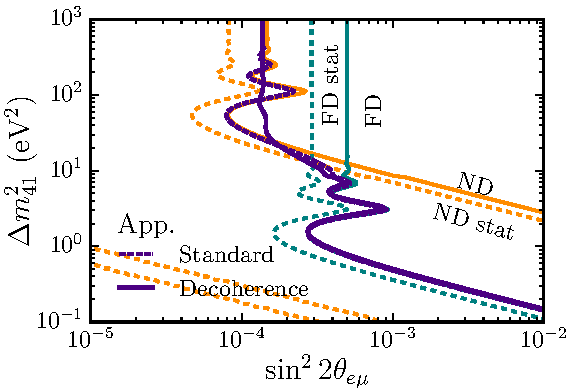
\includegraphics[width=0.49\textwidth]{figs/NDFD_Shape_app.pdf}
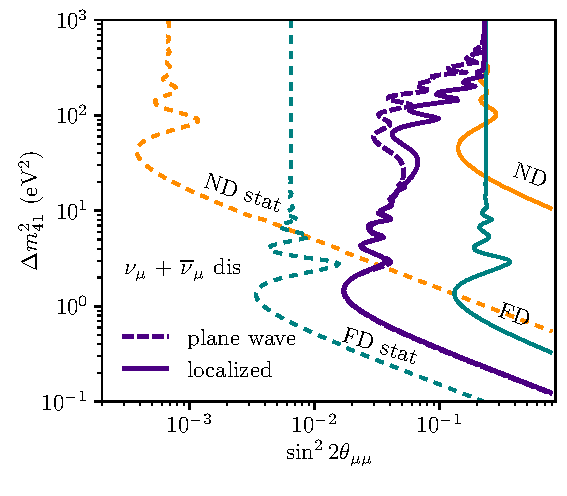
\includegraphics[width=0.49\textwidth]{figs/NDFD_Shape_dis.pdf}
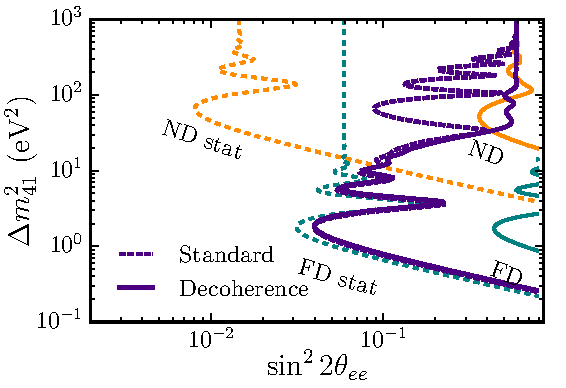
\includegraphics[width=0.49\textwidth]{figs/NDFD_Shape_edis.pdf}
\caption{Appearance (a) and disappearance (b) sensitivities to the phenomenological parameters $\theta_{\mu \mu}$ and $\theta_{e \mu}$ at \nus. The orange and light blue curves assume only a single near and a far detector, respectively, and do not take decoherence into account. The solid and dashed purple curves assume the presence of both detectors. %Correlated and uncorrelated flux systematics between detectors are both taken to be 0.5 \%. Cross sections $\times$ efficiencies uncertainties are 20\% and background errors 35 \%.
\label{fig:3+1sens}}
\end{figure}
%

\begin{figure}
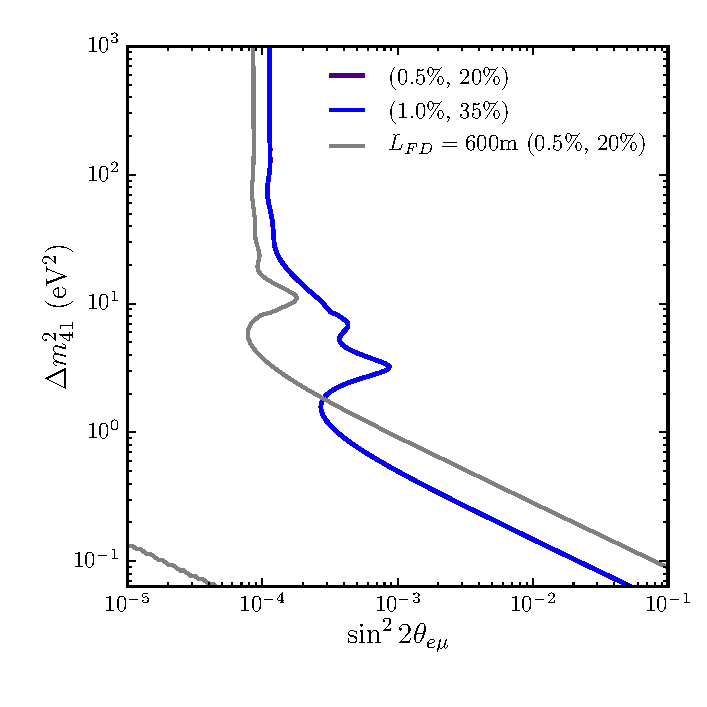
\includegraphics[width=0.49\textwidth]{figs/Comparison_app.pdf}
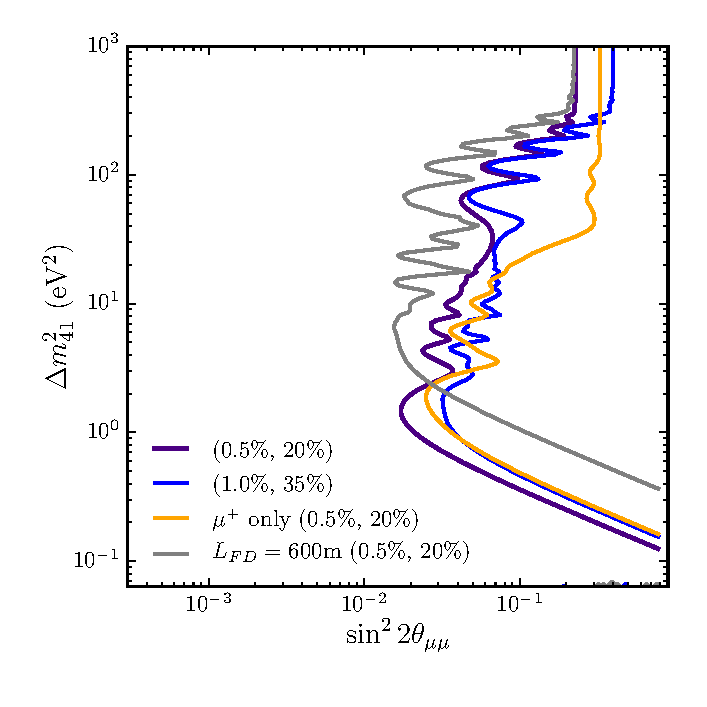
\includegraphics[width=0.49\textwidth]{figs/Comparison_dis.pdf}
\caption{Appearance (a) and disappearance (b) sensitivities to the phenomenological parameters $\theta_{\mu \mu}$ and $\theta_{e \mu}$ at \nus for far detector distances of 2 km and 600 m. We also show the recent SBN analysis in \cite{Cianci2017} and IceCUBE bounds \cite{TheIceCubeCollaboration2016} \label{fig:3+1comp}.}
\end{figure}
%
In this section we present the results of our sensitivity analysis for \nus, for which we used the GLoBES package \cite{Globes2005}. We start by noting that in an experiment like \nus, the charge identification of muons is extremely important to separate neutrino and antineutrino events in the detectors. This is true independently of whether we are interested in oscillation analyses or cross section measurements. For instance, in an $\nu_{e} \to \nu_{\mu}$ appearance experiment, the greatest source of background comes from the misidentified intrinsic antineutrinos in the $\overline{\nu}_{\mu} \to \overline{\nu}_{\mu}$ channel. This, however, can be circumvented with large enough magnetic fields at the detectors and curvature analyses of the muon tracks. In all our simulations we assume that both the near and far detectors are magnetised. More specifically, we implement migration matrices from the SuperBIND style iron-scintillator detector, which have kindly been provided to us by the collaboration~\footnote{Ryan Bayes, private communication}. The far detector is assumed to have a fiducial mass of 1.3 kt, whilst the near detector is taken to be a smaller version of it with 0.2 kt of fiducial mass.  

\subsection{Systematics Implementation \label{sec:appendix_sys}}

Here, we detail our methodology for dealing with systematics errors at \nus. We choose to use the pull method, which adds penalties to the best-fit parameter when deviating the parameters that control the systematics away from their central values. We work with a $\chi^2$ test which can be written as
%
\begin{equation}
\chi^2 _{\text{TOT}} = \sum_{D} \sum_{C} \chi^2_{D, C} + \chi^2_{\text{Pull}}.
\end{equation}
%
The $\chi^2_{D, C}$ for each detector $D$ and channel $C$ is a sum over the energy bins $E_i$ and a function of theoretical event rate $T^i_{D, C}$ and the simulated observed rate $O^i_{D, C}$:
%
\begin{equation}
\chi^2_{D, C} = 2 \sum_{i}^{n_{\text{bins}}} \Big(T^i_{D, C} - O^i_{D, C} + O^i_{D, C} \ln{\frac{O^i_{D, C}}{T^i_{D, C}}}\Big).
\end{equation}
%
The set of systematical errors for the signal and the background are represented by auxialiary parameters $\alpha$ and $\beta$, respectively, and are to be profiled over when calculating the theoretical event rates
%
\begin{align}
T^i_{D, C} =& (1 + \alpha_{\text{Flux}}^C + \alpha_{\text{Det}}^D + \alpha_{\text{Xsec}}^{i, C}) S^i_{D, C} + (1 + \beta^{D,C}) B^i_{D, C},
\end{align}
%
where $S^i_{D, C}$ and $B^i_{D, C}$ are the signal and background in the $i$-th energy bin, respectively. The error $\alpha_{\text{Flux}}^C$ is the total flux normalization error, correlated between near and far detector,  $\alpha_{\text{Det}}^D$ are the uncorrelated detector specific systematics and $\alpha_{\sigma_C}^i$ are the bin dependent cross sections and efficiency errors, which take shape uncertainties into account. We emphasize that the total flux normalization for the channels of interest is only uncorrelated between the two flux components. For examaple, for a $\pi^+$ polarity run, we have:
%
\begin{eqnarray}
\alpha_{\text{Flux}}^{\nu_{e} \to \nu_{\mu}} = \alpha_{\text{Flux}}^{\overline{\nu}_{\mu} \to \overline{\nu}_{\mu}} & =  \alpha_{\text{Flux}}^{\mu^+}, \quad  \alpha_{\text{Flux}}^{\nu_{\mu} \to \nu_{\mu}}  =  \alpha_{\text{Flux}}^{\pi^+}.
\end{eqnarray}
%
The background systematics take into account an overall normalization factor uncorrelated amongst all channels and detectors with $\beta_{BG}^{D,C}$ and shape effects with $\beta_{BG}^{i}$, also uncorrelated for all channels and detectors. Depending on what channel we are considering, there will be cross section uncertainties in the charge misidentificiation component of the background, which are taken into account in our analysis but not included in this discussion. In total, for our 4 channels of interest, 16 energy bins and one beam polarity, we have 52 signal systematic errors and 8 for the background.

In all our results, except when explicitly stated otherwise, we include 0.5\% flux normalisation uncertainties correlated between near and far detectors, and 0.5\% for detector specific uncertainties. Bin dependent cross section times efficiency uncertainties are taken to be 20\% at the time of the measurement, and overall background normalisation uncertainties 35\%. We also include an energy calibration error of 0.5\%. Finally, we point out that the $\chi^2$ analysis is done for the far and near detectors datasets, without resorting to near to far ratios.
 
\subsubsection{3+1 Model}

For easier comparison with other studies, we choose to work with the 3+1 phenomenological parameters $\sin^2{2 \theta_{\alpha \beta}} = 4 |U_{\alpha 4}|^2|U_{\beta 4}|^2$ and $\sin^2{2 \theta_{\alpha \alpha}} = 4|U_{\alpha 4}|^2(1 - |U_{\alpha 4}|^2)$. Figure \ref{fig:3+1sens} shows the sensitivity of \nus to the phenomenological parameters in the 3+1 model. We show the curve including the decoherence treatment and the one using the plane wave formulae. 

The interplay between the near and the far detectors in this study is pivotal and has been studied in the literature before in the context of VLENF \cite{Winter2012a}. For low $\Delta m^2_{41}$, the near detector is not affected by oscillations and can safely measure cross sections and the flux normalisation, whilst the far detector measures the oscillation parameters. The detector roles are swapped for larger $\Delta m^2_{41}$, however, where oscillations now develop at the near detector and are already washed out at the far detector. In fact, due to decoherence effects, the oscillations are washed out at the near detector in this region anyway. 


In figure \ref{fig:3+1comp}, we compare \nus exclusion curves to the recent analysis of SBN \cite{Cianci2017}, and overlay the IceCUBE bounds\cite{TheIceCubeCollaboration2016}. One sees that whilst one does not need an experiment like \nus to test lower mass regions, it does perform much better than any other experiment for larger masses, where the measurement is essentially one of the zero-distance effects of the non-unitarity of the PMNS matrix. For this reason, we show the sensitivity of an alternative setup of \nus, where we put the far detector at a distance of $600$ m, which strengthens this aspect of the sterile search. 

We show the set of bounds coming from oscillation experiments and beta decay experiments in figure \ref{fig:bounds}. We only show appearance bounds for electron-muon or the inverse channel. The different beta decay bounds correspond to the following radioactive isotopes: 1 -- $^3$H, 2 -- $^3$H, 3 -- $^{187}$Re, 4 -- $^3$H, 5 -- $^3$H, 6 -- $^{63}$Ni, 7 -- $^{63}$Ni, 8 -- $^{35}$S, 9 -- $^{64}$Cu, 10 -- $^{20}$F. The bound labelled 11 is from the Troitsk nu-mass experiment as reported in Ref.\cite{Abdurashitov:2017kka}
%
As these experiments measure slighly different combinations of matrix elements, we show the bounds under two assumptions. In the first case we assume comparable mixings between the fourth mass state and all flavours, $|U_{e4}| = |U_{\mu 4}|$. In the second, we make no such assumption, instead using the relation $|U_{e4}U_{\mu 4}|\le |U_{e4}|\sqrt{1-|U_{e4}|^2}$ which weakens the bounds from electron only experiments significantly.

\begin{figure*}
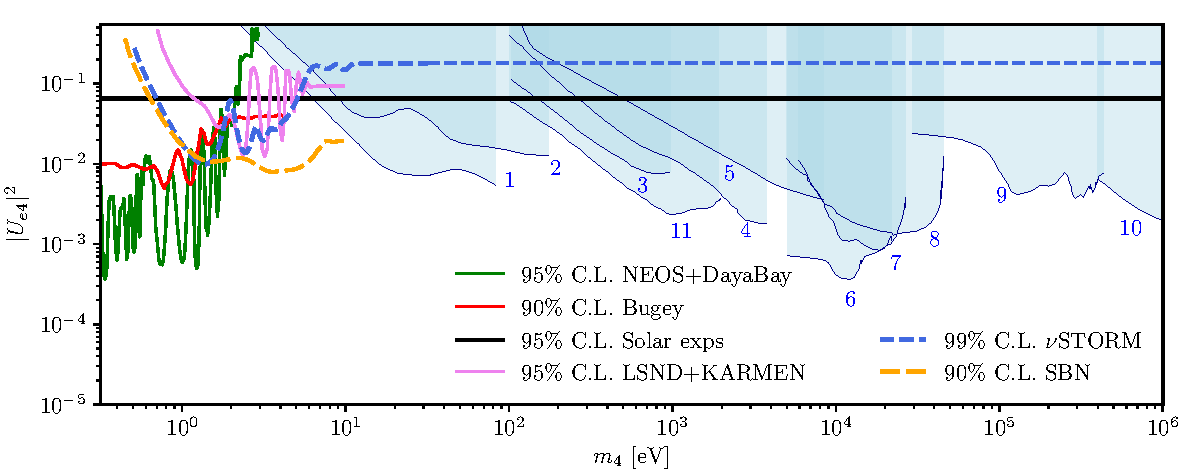
\includegraphics[width=\textwidth]{figs/Bounds_edis.pdf}
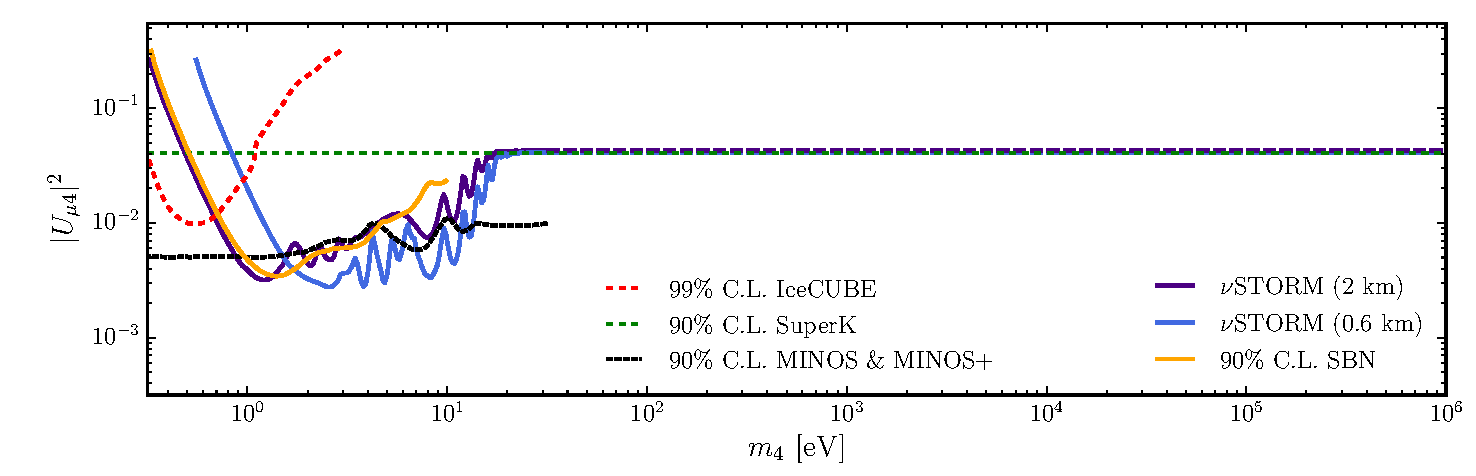
\includegraphics[width=\textwidth]{figs/Bounds_dis.pdf}
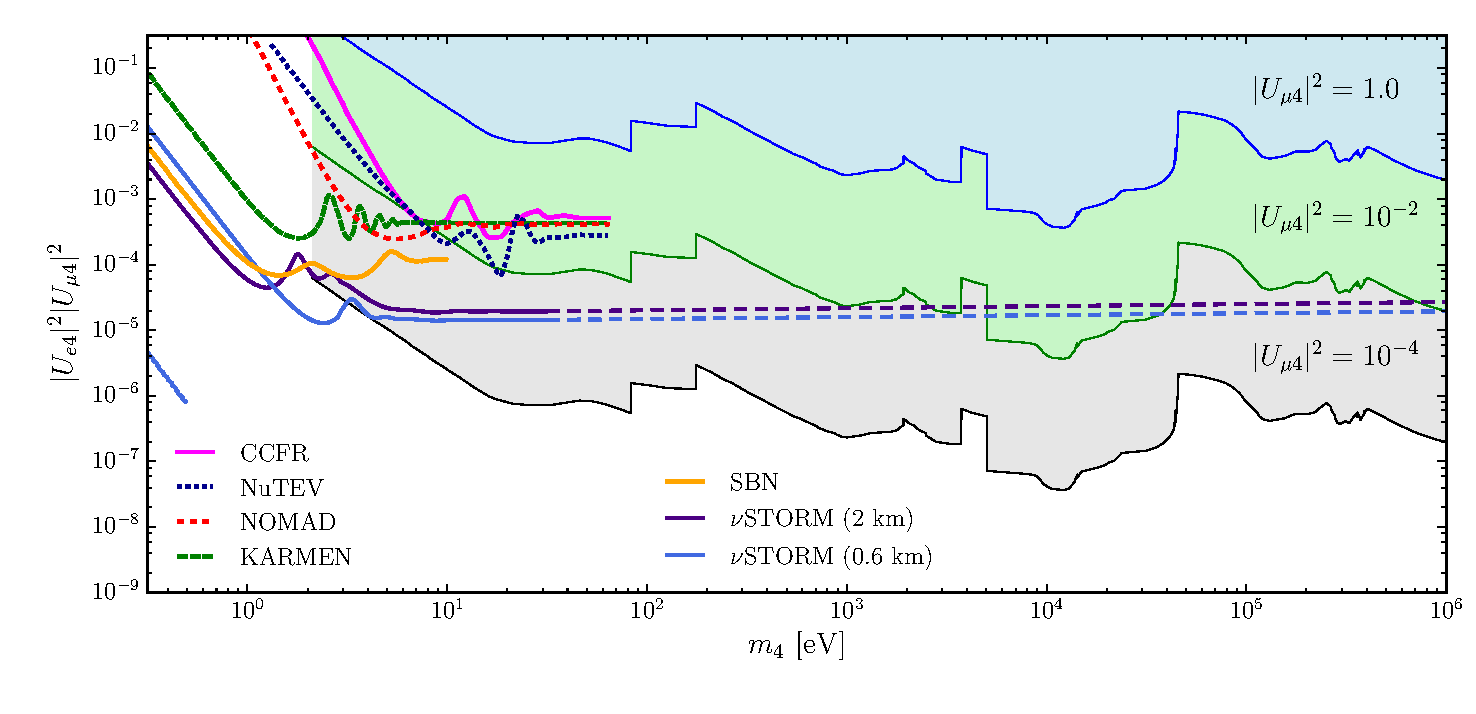
\includegraphics[width=\textwidth]{figs/Bounds_UeUmuapp.pdf}
\caption{ Bounds on the electron-sterile mixing for different values of the muon-sterile mixing. The numbered bounds labels follow the sequence in \cite{Dragoun2015} and 11 comes from \cite{Abdurashitov:2017kka}. All bounds are at 95\% C.L., except 2 and 9, which are at 90\%. The past accelerator experiment bounds were taken from \cite{Astier2003} for NOMAD and CCFR, and from \cite{Avvakumov2002} for NuTEV and KARMEN, all at 90\% C.L. The SBN \cite{Cianci2017} and the two $\nu$STORM bounds with different far detector distances are the expected limits at 90\% C.L.\label{fig:bounds}}
\end{figure*}


\subsubsection{3+2 Model}

	We now present our results for the 3+2 model. In this case, the ordering of the two sterile neutrinos is non physical, hence $\Delta m^2_{54} > 0 $ without any loss of generality. Note that now the presence of two oscillation frequencies somewhat spoils the interplay of the near and far detectors mentioned above. If $\Delta m^2_{41}$ is in the $\mathcal{O}(1)$ ev$^2$ region and $\Delta m^2_{51}$ in the $\mathcal{O}(10^2)$ ev$^2$ region, then both the near and the far detectors are affected by oscillations and the systematics cannot be safely measured in any detector.
	
	Some of the bounds that \nus would be able to place on the 3+2 parameters are shown in figure \ref{fig:3+2sens_dis} for a disappearance only experiment, and in figure \ref{fig:3+2sens_app} for an appearance experiment. We emphasise that these bounds are extremely model dependent, and that if one was to marginalise over the extra "spectator" parameters then the null hypothesis is almost always allowed. The values chosen for the extra parameters in each plot is motivated by the global fit in \cite{Collin2016a}.

% \begin{figure*}[t]
% \centering
% %All the original file paths were like the one below instead of "code/coh_5_ND/"
% %\includegraphics[width=0.33\textwidth]{../../5_neutrinos_myprob/UUvsUU/Plots/Dis_dm_UU_v1.pdf}
% \includegraphics[width=0.33\textwidth]{code/coh_5_ND/Plots/Dis_dm_UU_v1.pdf}
% }
% \subfloat[]{
% 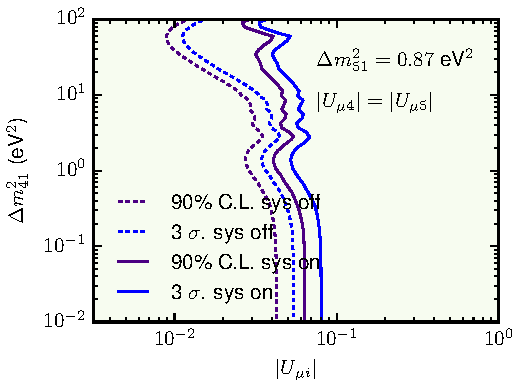
\includegraphics[width=0.33\textwidth]{code/coh_5_ND/Plots/Dis_dm_UU_v2.pdf}
% } 
% \subfloat[]{
% \includegraphics[width=0.33\textwidth]{code/coh_5_ND/Plots/Dis_dm_UU_UU.pdf}
% }
% \caption{Sensitivity of NuSTORM to 3+2 oscillation parameters for a disappearance experiment. In each plot, we bound the combination of parameters in the x and y axes using assumptions that are show in the legend. The shading corresponds to the $\chi^2$ surface in the systematics off case, with darker regions representing larger $\chi^2$'s.\label{fig:3+2sens_dis} }
% \end{figure*}

\begin{figure}
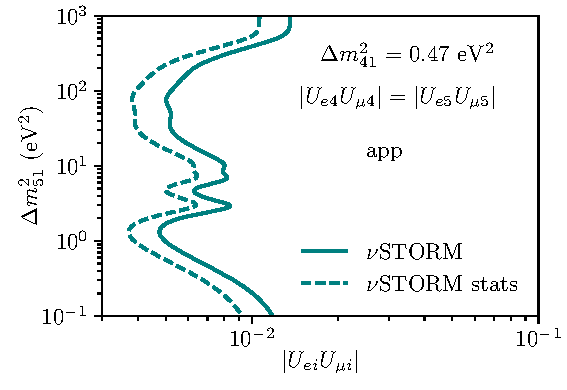
\includegraphics[width=0.49\textwidth]{figs/App_dm_UU.pdf}
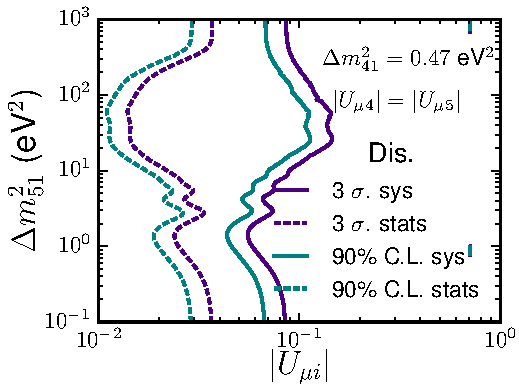
\includegraphics[width=0.49\textwidth]{figs/Dis_dm_UU.pdf}
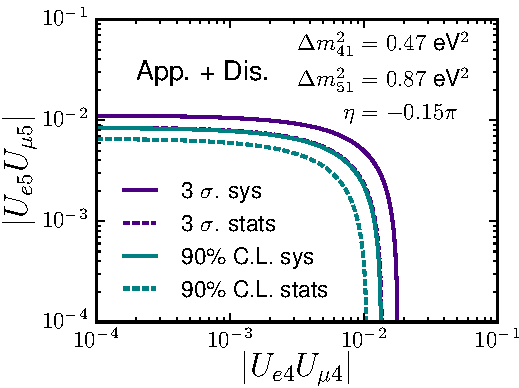
\includegraphics[width=0.49\textwidth]{figs/App_dm_UU_UU.pdf}
\caption{Same as before but for an appearance experiment. In (b) we perform a combined analysis of appearance and disappearance data. The allowed regions found by J. Kopp et al in \cite{Kopp2013} are shown in dark green regions. \label{fig:3+2sens_app} }
\end{figure}


\subsubsection{Precision Measurements and CPV}

	In the previous section we explored the sensitivity of \nus to the 3+2 parameters, but in this section we assume a signal and explore its consequences. In particular, we look at the sensitivity of \nus to the effective CP violation phase $\eta$. This is to be contrasted with the study in \cite{DeGouvea2015a}, where the CP violation arises from the interference between the $\Delta m^2_{31}$ and $\Delta m^2_{41}$ mass differences. In our study, the CP violation arises exclusively due to the interference between the two active-sterile oscillations.

	Assuming a precision of 10\% and 20\% in the measurement of the 3+2 model parameters, we evaluate the sensitivity to $\eta$ in figure \ref{fig:CP1D}, showing that \nus could be sensitive to maximally CP violating phases at 3 and 4 $\sigma$'s.  


\begin{figure}[t!]
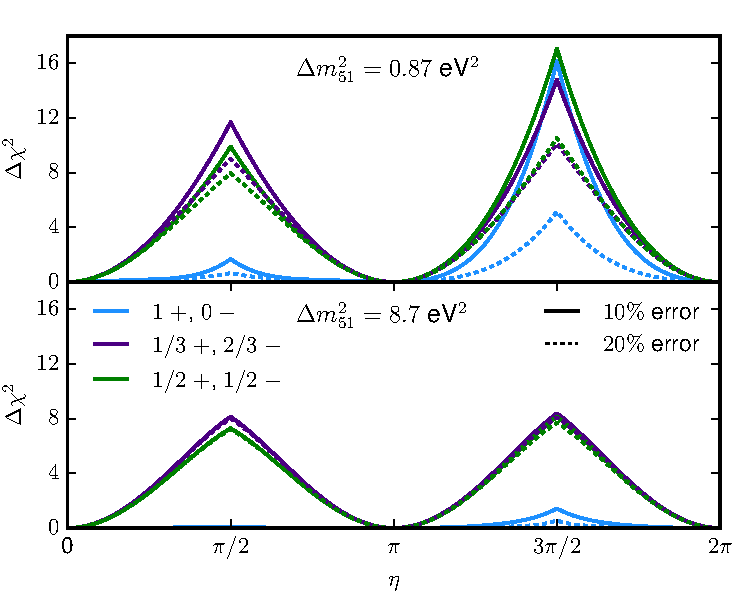
\includegraphics[width=0.49\textwidth]{figs/CP_sensitivity.pdf}
\caption{The sensitivity of \nus to the CP violating phase $\eta$ when giving all other parameters $10 \%$ and $20 \%$ errors. In (a) $\Delta m^2_{51} = 0.87 $ eV$^2$, whilst in (b), we use a ten times larger value. We use three different configurations: 100\% $\mu^+$  runtime, 66\% $\mu^-$ and 33\% $\mu^+$ runtime, and 50\% runtime each. The other parameters in the 3+2 model are assumed to be $\Delta m^2_{41} = 0.47 $ eV$^2$, $|U_{e4}|=0.13$, $|U_{e5}|=0.14$, $|U_{\mu4}|=0.15$ and $|U_{\mu5}|=0.13$. \label{fig:CP1D}}
\end{figure}


\subsection{Averaged Out Steriles}

In this section I show the results I had obtained some time when bounding non-unitarity as it is interpreted in \cite{Ross-Lonergan2016}. 

The oscillation probability for active neutrinos can be written as
\begin{align} \label{eq:general_prob}
P_{\nu_{\alpha} \to \nu_{\beta}}= \left| \sum_k^3 U_{\alpha k}^* U_{\beta k} \right|^2 - & 2 \sum_{k>j}^{3} \Re(U_{\alpha k}^* U_{\beta k} U_{\alpha j} U_{\beta j}^*)\, (1 - \Re(I_{k j})) \\\nonumber -& 2\sum_{k>j}^{3} \Im(U_{\alpha k}^* U_{\beta k} U_{\alpha j} U_{\beta j}^*) \Im(I_{k j}),
\end{align}
which at zero-distance ($L_{\text{osc}}$ due to atmospheric and solar mass-splittings is much larger than the baselines we are considering) becomes
\begin{align} \label{eq:general_prob}
P_{\nu_{\alpha} \to \nu_{\beta}}= \left| \sum_k^3 U_{\alpha k}^* U_{\beta k} \right|^2
\end{align}
For unitary mixing and no averaged out sterile neutrino, we expect the probability above to be equal to $\delta_{\alpha \beta}$. If we are dealing with a sterile neutrino whose oscillations have long been averaged out, then $P_{\alpha \to \beta}$ can deviate from 0 or 1 in the way we demonstrated in the previous sections. In that case we can bound this deviation by looking for ``zero"-distance flavour transitions. 

The bounds we place are all on the assumption that the oscillation probability is either 0 or 1, where $\nu$STORM would be probing a constant normalization in its event rates. The results shown in \ref{fig:non-uni} for $\nu$STORM are compared with the analysis in MiniBoone \cite{Karagiorgi2010} and SBN\footnote{Through private communication, Mark has claimed that he and Giorgia do not trust the SBN results anymore. It is not clear why, but it seemed like the assumption of unitarity in MC generators made their result unreliable.} (taken from a talk given at Fermilab \cite{Ross-Lonergan2016}).

\begin{figure}
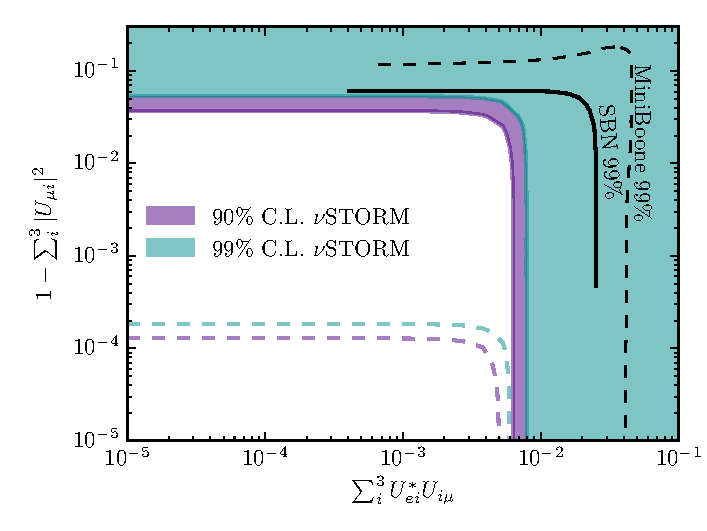
\includegraphics[width=0.49\textwidth]{figs/Averaged_joined.pdf}
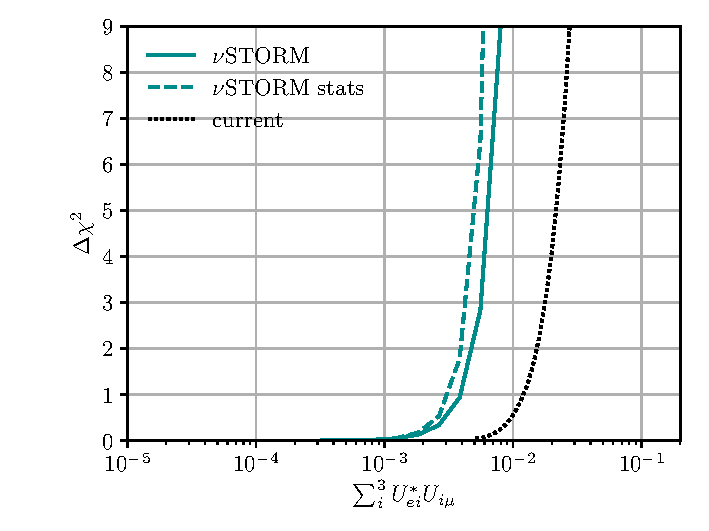
\includegraphics[width=0.49\textwidth]{figs/Averaged_1D_app.pdf}
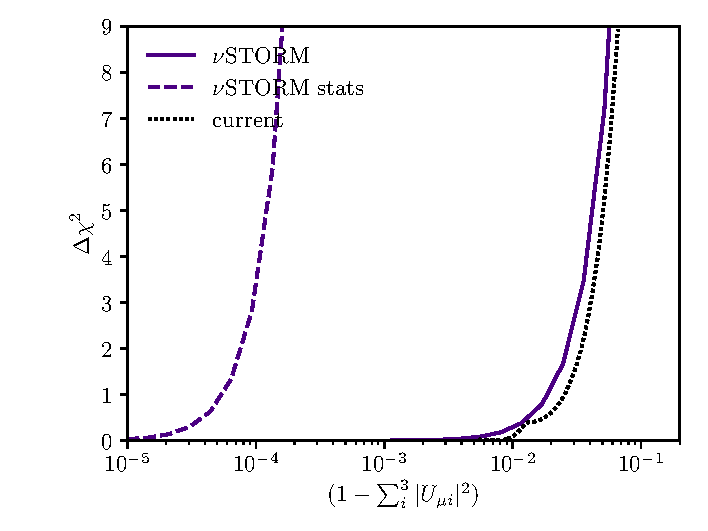
\includegraphics[width=0.49\textwidth]{figs/Averaged_1D_dis.pdf}
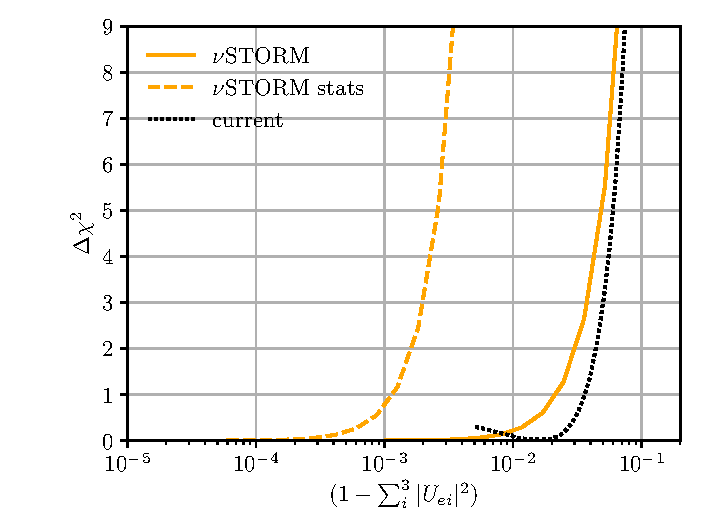
\includegraphics[width=0.49\textwidth]{figs/Averaged_1D_edis.pdf}
\caption[Bounds and sensitivity of $\nu$STORM to averaged out sterile neutrinos.]{Bounds on the non-unitarity of the mixing matrix in the averaged out sterile oscillation sense. Top left shows the two dimensional plane HEHEHEHEHEEHEHEHEHEHEH experiments.\label{fig:non-uni}}
\end{figure}

It is important to note that the bounds we just placed can be translated into model dependent bounds on the active-sterile mixing angle using expressions given earlier in these notes.

\subsection{MUV}

If we want to explore the transition the regions we just discussed, it is instructive to constrain the MUV unitarity at $\nu$STORM as well. This will  be very similar to the previous analysis, however, different normalization factors are required depending on the production process of the neutrino. For this reason, we define an effective flavour transition probability which absorbs any factors due to non-unitarity at production and detection.

\begin{equation}
 \hat{P}_{\nu_{\alpha} \to \nu_{\beta}} = \frac{\sigma^{\text{CC}}_{\alpha}}{\sigma^{\text{CC (SM)}}_{\alpha}} \, P_{\nu_{\alpha} \to \nu_{\beta}} \, \frac{d\Phi^{\text{CC}}_{\alpha}/dE}{d\Phi^{\text{CC (SM)}}_{\alpha}/dE},
\end{equation}
where $P_{\nu_{\alpha} \to \nu_{\beta}}$ is the standard MUV flavour transition probability.

The non-unitarity of the mixing matrix $N$ can be parametrized in different ways. Here, we choose to use a lower triangular matrix $\boldsymbol{\alpha}$ following Blennow et al \cite{Blennow2016}:
\begin{equation}
 N = (\boldsymbol{1} - \boldsymbol{\alpha}) U,
\end{equation}
where $U$ is the standard (nearly?) unitary PMNS matrix and 
\[
\boldsymbol{\alpha} =
  \begin{pmatrix}
    \alpha_{e e} & 0 & 0 \\
    \alpha_{\mu e} & \alpha_{\mu \mu} & 0 \\
    \alpha_{\tau e} & \alpha_{\tau \mu} & \alpha_{\tau \tau} \\
  \end{pmatrix},
\]
with real diagonal entries. Using the previous parametrization one can then write the quantity of interest $NN^{\dagger}$ as
\begin{equation}
 NN^{\dagger} = \boldsymbol{1} - \boldsymbol{\alpha} - \boldsymbol{\alpha}^{\dagger} + \boldsymbol{\alpha}\boldsymbol{\alpha}^{\dagger},
\end{equation}
yielding (omitting the inaccessible entries)
\[
NN^{\dagger} =
  \begin{pmatrix}
    1 - 2\alpha_{e e} +\alpha_{e e}^2 & \alpha_{\mu e}^*(\alpha_{ee}-1) & - \\
    \alpha_{\mu e}(\alpha_{ee}-1) & 1 - 2\alpha_{\mu \mu} + \alpha_{\mu \mu}^2 + |\alpha_{\mu e}|^2 & - \\
    - & - & - \\
  \end{pmatrix}.
\]
Alternatively, one can parametrize $N$ as $N = \boldsymbol{T} U$, where we use the matrix $\boldsymbol{T}$ from Escrihuela et al \cite{Escrihuela2015}, which is written as
\[
\boldsymbol{T} =
  \begin{pmatrix}
    \alpha_{11} & 0 & 0 \\
    \alpha_{21} & \alpha_{22} & 0 \\
    \alpha_{31} & \alpha_{32} & \alpha_{33} \\
  \end{pmatrix}.
\]
In this parametrization, the quantity of interest $NN^{\dagger}$ is slightly simpler
\[
NN^{\dagger} =
  \begin{pmatrix}
    \alpha_{11}^2 & \alpha_{11}\alpha_{21}^* & - \\
    \alpha_{11}\alpha_{21} & \alpha_{22}^2 + |\alpha_{21}|^2 & - \\
    - & - & - \\
  \end{pmatrix},
\]
where the relation between the two parametrizations is clear: $\alpha_{\alpha \beta} \to \delta_{ij} - \alpha_{ij}$, with $e \to 1, \mu \to 2$ and $\tau \to 3$. In table \ref{tab:PeffectiveNuSTORM}, we list the different channels at $\nu$STORM and the effective flavour transition probabilities associated with them in the different parametrizations.
\renewcommand{\arraystretch}{0.4}
\begin{table}[h]
\begin{tabular}{lllll}
P&Channel& $\hat{P}_{\nu_{\alpha} \to \nu_{\beta}}^{3+1}$
& $\hat{P}_{\nu_{\alpha} \to \nu_{\beta}}^{\text{Blennow et al}} $&  $\hat{P}_{\nu_{\alpha} \to \nu_{\beta}}^{\text{Escrihuela et al}}$ \\
%
\hline
%
$\pi^+$ &$\nu_{\mu} \to \nu_{\mu} $&$1 - 2 |U_{\mu 4}|^2 + |U_{\mu 4}|^4 $&$((1-\alpha_{\mu \mu})^2+|\alpha_{\mu e}|^2)^2 $ & $(\alpha_{22}^2+|\alpha_{21}|^2)^2 $\\
%
\cline{2-5}
%
&$\nu_{\mu} \to \nu_{e}$&$|U_{e 4}|^2|U_{\mu 4}|^2$&$ (1-\alpha_{ee})^2|\alpha_{\mu e}|^2 $&$\alpha_{11}^2|\alpha_{21}|^2$\\
 \hline
 %
 %
$\mu^+ $ & $\nu_{e} \to \nu_{e}$&$\left(1 - 2 |U_{e 4}|^2 + |U_{e 4}|^4\right) \left( 1 - |U_{\mu4}|^2\right) $ & $(1-\alpha_{e e})^4 ((1 - \alpha_{\mu \mu})^2 +|\alpha_{\mu e}|^2)$ & $\alpha_{11}^4(\alpha_{22}^2+|\alpha_{21}|^2)$\\
%
\cline{2-5}
%
&$\overline{\nu}_{\mu} \to \overline{\nu}_{\mu}$&$\left(1 - 2 |U_{\mu 4}|^2 + |U_{\mu 4}|^4\right) \left( 1 - |U_{e4}|^2\right)$ & $((1 - \alpha_{\mu \mu})^2 +|\alpha_{\mu e}|^2)^2(1-\alpha_{e e})^2$ & $(\alpha_{22}^2 +|\alpha_{21}|^2)^2\alpha_{11}^2$\\
%
\cline{2-5}
%
&$\nu_{e} \to \nu_{\mu}$ & $|U_{e 4}|^2|U_{\mu 4}|^2\left( 1 - |U_{\mu4}|^2\right)$ & $(1-\alpha_{ee})^2|\alpha_{\mu e}|^2((1 - \alpha_{\mu \mu})^2 +|\alpha_{\mu e}|^2)\,$&$\alpha_{11}^2|\alpha_{21}|^2(\alpha_{22}^2+|\alpha_{21}|^2)$\\
\end{tabular}
\caption{\label{tab:PeffectiveNuSTORM}Comparison of the effective flavour transition probability for the 3+1 model ($m_4 > m_{\pi^{\pm}}$) and the two parametrizations for the non-unitarity of the mixing matrix (Blennow et al \cite{Blennow2016} and Escrihuela et al \cite{Escrihuela2015})}
\end{table}

% 
% \begin{itemize}
%  \item \underline{$\pi^+ \to \mu^+ \nu_{\mu}$:}
%       \begin{align*}
% 	\hat{P}_{\nu_{\mu} \to \nu_{\mu}} &= 1 - 2 |U_{\mu 4}|^2 + |U_{\mu 4}|^4, \\
% 	\hat{P}_{\nu_{\mu} \to \nu_{e}} &= |U_{e 4}|^2|U_{\mu 4}|^2.
%       \end{align*}
%  \item \underline{$\mu^+ \to e^+ \nu_{e} \overline{\nu}_{\mu}$:}
%       \begin{align*}
% 	\hat{P}_{\nu_{e} \to \nu_{e}} &= \left(1 - 2 |U_{e 4}|^2 + |U_{e 4}|^4\right) \left( 1 - |U_{\mu4}|^2\right), \\	
% 	\hat{P}_{\overline{\nu}_{\mu} \to \overline{\nu}_{\mu}} &= \left(1 - 2 |U_{\mu 4}|^2 + |U_{\mu 4}|^4\right) \left( 1 - |U_{e4}|^2\right), \\
% 	\hat{P}_{\nu_{e} \to \nu_{\mu}} &= |U_{e 4}|^2|U_{\mu 4}|^2\left( 1 - |U_{\mu4}|^2\right).
%       \end{align*}
% \end{itemize}

One can see that in the MUV regime, the different oscillation channels are now dependent on mixing that might not even involve the neutrino (low energy) flavours. It is curious that at $\nu$STORM, the channels $\nu_{\mu} \to \nu_{\mu}$ and $\overline{\nu}_{\mu} \to \overline{\nu}_{\mu}$ are dependent on different mixings, since they involve neutrinos with different parent particles. In fact, one could hope to constrain $|U_{e4}|^2$ when measuring the two channels. Naively, one hopes for a cancellation similar to the near to far ratio, cancelling the dependence on cross sections and on the mixing $|U_{\mu4}|^2$ when bounding the ratio
\[ \frac{ N_{ \overline{\nu}_{\mu} \to \overline{\nu}_{\mu}}}{N_{ \nu_{\mu} \to \nu_{\mu}}} .\]

\begin{figure}
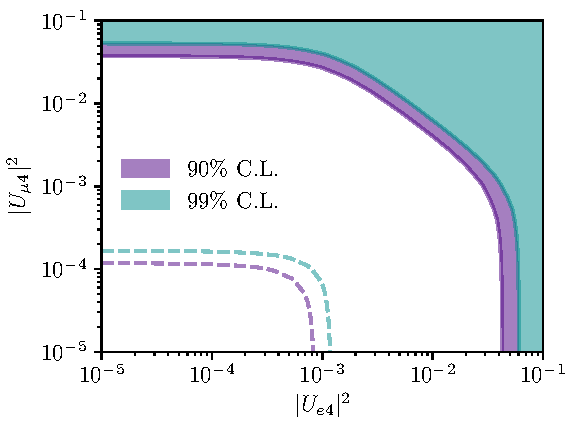
\includegraphics[width=0.49\textwidth]{figs/MUV_joined.pdf}
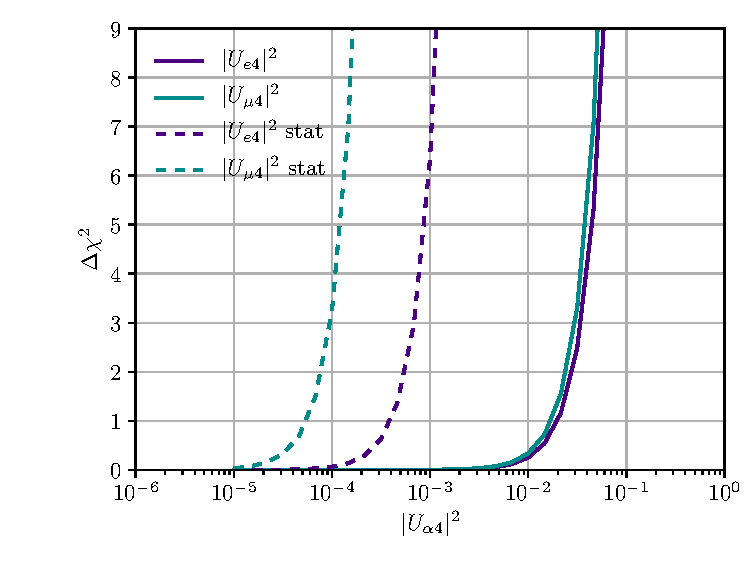
\includegraphics[width=0.49\textwidth]{figs/MUV_1D.pdf}
\caption{Bounds on the non-unitarity of the mixing matrix in the averaged out sterile oscillation sense. \label{fig:non-uni}}
\end{figure}


\section{Overview}

All the great things we concluded in this wonderful study.
